The amount of data Axpo required to migrate is huge and highly heterogeneous and not much information are available for such amount and complexity.
A large number of papers has been published regarding migrations to the Cloud, but few are relevant with this project.

The following publications are the most relevant regarding the migration process carried out by Axpo.

\paragraph{Architecture design}
    Some publications focus on systematic architecture design techniques, starting from the target domain \cite{bib:related_work:books:architecture}.
    The design proposed is, however, too much formal and high-level: the document focuses on understanding the needs of the company to choose which components are needed in the Cloud architecture.
    The needs are however described in a high-level notation, as shown in Figure \ref{fig:related:architecture_high_level}.
    Depending on the identified requirements, different rules are applied.
    These rules are used for specifying software architecture dependencies.
    For example, one of the rules is:
        \begin{center}
            \texttt{
                If AD HOC ANALYSIS is selected then enable INFORMATION VIRTUALIZATION on component INFORMATION MANAGEMENT SERVER.
            }
        \end{center}
    
    This design is meant for engineering a whole software architecture from scratch, not just for re-engineering a single component (in this case, the analytical back-end) while leaving the others unchanged.
    Moreover, the company was already aware of their needs, since they were the same of the on-premise structure.
    
    \begin{figure}
        \centering
        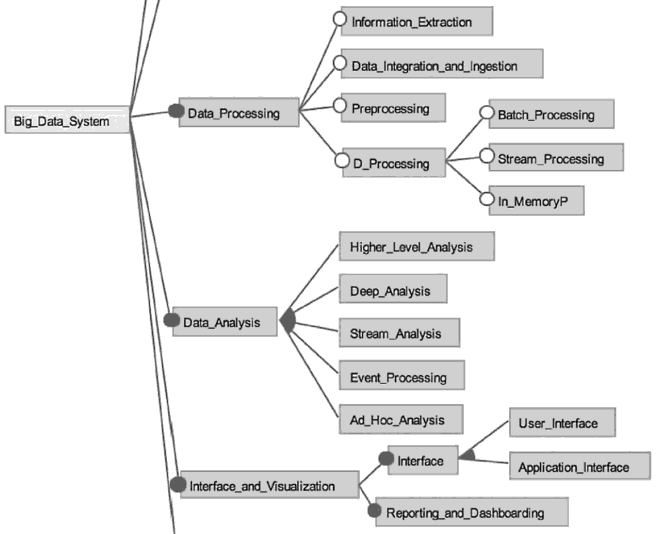
\includegraphics[width=.8\textwidth]{res/relatedwork/architecture_high_level.png}
        \caption{High-level architecture design \cite{bib:related_work:books:architecture}.}
        \label{fig:related:architecture_high_level}
    \end{figure}
    
    Issues relevant to the re-engineering process required by Axpo are also mentioned, such as the need to perform cleaning operations on data, but are not investigated or described in detail.

\paragraph{Migration process}
    Other publications focus on the re-engineering process itself, as well as some expected issues \cite{bib:related_work:books:migration}.
    The document, however, presents only a brief description of each problem, inviting readers to carry out further analyses on their own.
    The issues exposed in the publication have been also encountered during the migration process carried out by Axpo, and will be described in more details in the chapter \ref{section:etl} and in section \ref{section:dwh:remappings}.
    
    The publication also contains some remarks about potentialities offered by the Cloud, even though they are all discussed in general.
    Some of these aspects are also described in more details in this section and in chapter \ref{section:azure}.
    